
\gaokaoheader{2020}{天津卷}




\begin{enumerate}
\item
在物理学发展的进程中,人们通过对某些重要物理实验的深入观察和研究,获得正确的理论认识。下列
图示的实验中导致发现原子具有核式结构的是 \xzanswer{D} 
\pfourchoices
{\includesvg[width=4cm]{picture/svg/GZ-3-tiyou-0763}}
{\includesvg[width=4cm]{picture/svg/GZ-3-tiyou-0765}}
{\includesvg[width=4cm]{picture/svg/GZ-3-tiyou-0766}}
{\includesvg[width=4cm]{picture/svg/GZ-3-tiyou-0767}}






\item
北斗问天,国之夙愿。我国北斗三号系统的收官之星是地球静止轨道卫星,其轨道半径约为地球半径的$ 7 $倍。与近地轨道卫星相比,地球静止轨道卫星 \xzanswer{A} 
\begin{figure}[h!]
\centering
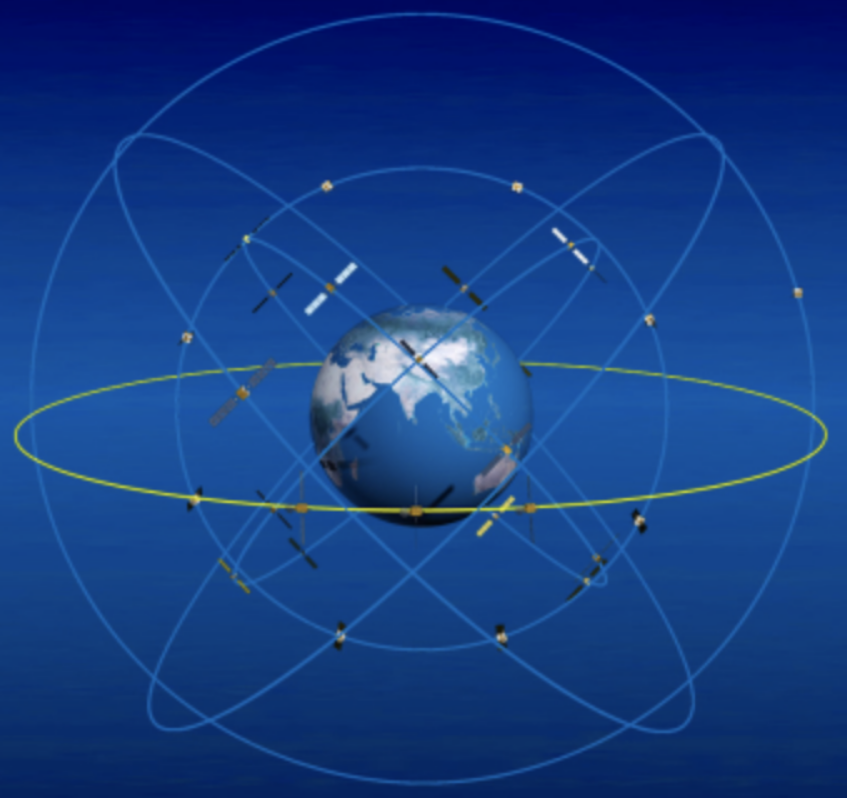
\includegraphics[width=0.2\linewidth]{picture/screenshot053}
\end{figure}


\fourchoices
{周期大}
{线速度大}
{角速度大}
{加速度大}




\item
新冠肺炎疫情突发,中华儿女风雨同舟、守望相助,筑起了抗击疫情的巍峨长城。志愿者用非接触式体
温测量仪,通过人体辐射的红外线测量体温,防控人员用紫外线灯在无人的环境下消杀病毒,为人民健康保驾护航。红外线和紫外线相比较 \xzanswer{B} 

\fourchoices
{红外线的光子能量比紫外线的大}
{真空中红外线的波长比紫外线的长}
{真空中红外线的传播速度比紫外线的大}
{红外线能发生偏振现象,而紫外线不能}




\item
一列简谐横波沿 $ x $ 轴正方向传播,周期为 $ T $, $ t=0 $ 时的波形如图所示。 $ t=\frac{T}{4} $时 \xzanswer{C} 
\begin{figure}[h!]
\centering
\includesvg[width=0.23\linewidth]{picture/svg/GZ-3-tiyou-0768}
\end{figure}

\fourchoices
{质点 $ a $ 速度方向沿 $ y $ 轴负方向}
{质点 $ b $ 沿 $ x $ 轴正方向迁移了 $ 1 \ m $}
{质点 $ c $ 的加速度为零}
{质点 $ d $ 的位移为$ -5 \ cm $}





\item
水枪是孩子们喜爱的玩具,常见的气压式水枪储水罐示意如图。从储水罐充气口充入气体,达到一定压
强后,关闭充气口。扣动扳机将阀门 $ M $ 打开,水即从枪口喷出。若在水不断喷出的过程中,罐内气体温
度始终保持不变,则气体 \xzanswer{B} 
\begin{figure}[h!]
\centering
\includesvg[width=0.23\linewidth]{picture/svg/GZ-3-tiyou-0769}
\end{figure}


\fourchoices
{压强变大}
{对外界做功}
{对外界放热}
{分子平均动能变大}








\item
手机无线充电是比较新颖的充电方式。如图所示,电磁感应式无线充电的原理与变压器类似,通过分别安
装在充电基座和接收能量装置上的线圈,利用产生的磁场传递能量。当充电基座上的送电线圈通入正弦式
交变电流后,就会在邻近的受电线圈中感应出电流,最终实现为手机电池充电。在充电过程中 \xzanswer{AC} 
\begin{figure}[h!]
\centering
\begin{subfigure}{0.4\linewidth}
\centering
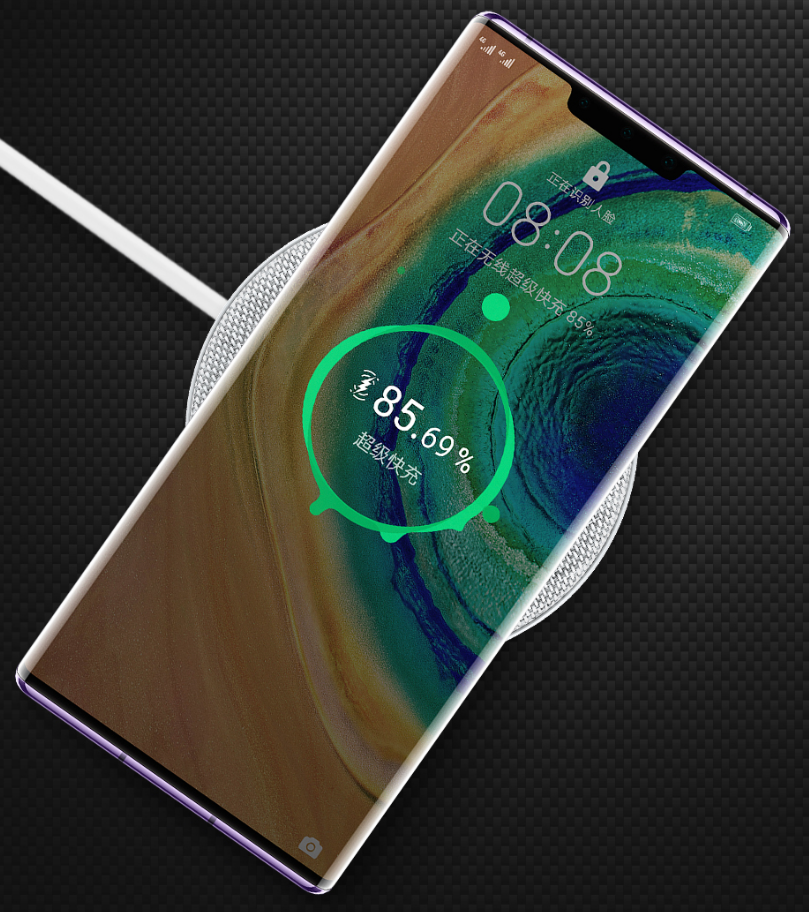
\includegraphics[width=0.3\linewidth]{picture/screenshot054}
\caption{}\label{}
\end{subfigure}
\begin{subfigure}{0.4\linewidth}
\centering
\includesvg[width=0.5\linewidth]{picture/svg/GZ-3-tiyou-0770} 
\caption{}\label{}
\end{subfigure}
\end{figure}


\fourchoices
{送电线圈中电流产生的磁场呈周期性变化}
{受电线圈中感应电流产生的磁场恒定不变}
{送电线圈和受电线圈通过互感现象实现能量传递}
{手机和基座无需导线连接,这样传递能量没有损失}





\item
如图所示,在 $ Oxy $ 平面的第一象限内存在方向垂直纸面向里,磁感应强度大小为 $ B $ 的匀强磁场。一带电
粒子从 $ y $ 轴上的 $ M $ 点射入磁场,速度方向与 $ y $ 轴正方向的夹角 $ \theta=45 ^{ \circ } $。粒子经过磁场偏转后在 $ N $ 点(图
中未画出)垂直穿过 $ x $ 轴。已知 $ OM=a $,粒子电荷量为 $ q $,质量为 $ m $,重力不计。则 \xzanswer{AD} 
\begin{figure}[h!]
\centering
\includesvg[width=0.2\linewidth]{picture/svg/GZ-3-tiyou-0771}
\end{figure}


\fourchoices
{粒子带负电荷}
{粒子速度大小为$\frac{q B a}{m}$}
{粒子在磁场中运动的轨道半径为 $ a $}
{$ N $ 与 $ O $ 点相距 $ (\sqrt{2}+1)a $}





\item
复兴号动车在世界上首次实现速度 $ 350 \ km/h $ 自动驾驶功能,成为我国高铁自主创新的又一重大标志性
成果。一列质量为 $ m $ 的动车,初速度为 $ v_{0} $,以恒定功率 $ P $ 在平直轨道上运动,经时间 $ t $ 达到该功率下的
最大速度 $ v_{m} $,设动车行驶过程所受到的阻力 $ F $ 保持不变。动车在时间 $ t $ 内 \xzanswer{BC} 
\begin{figure}[h!]
\centering
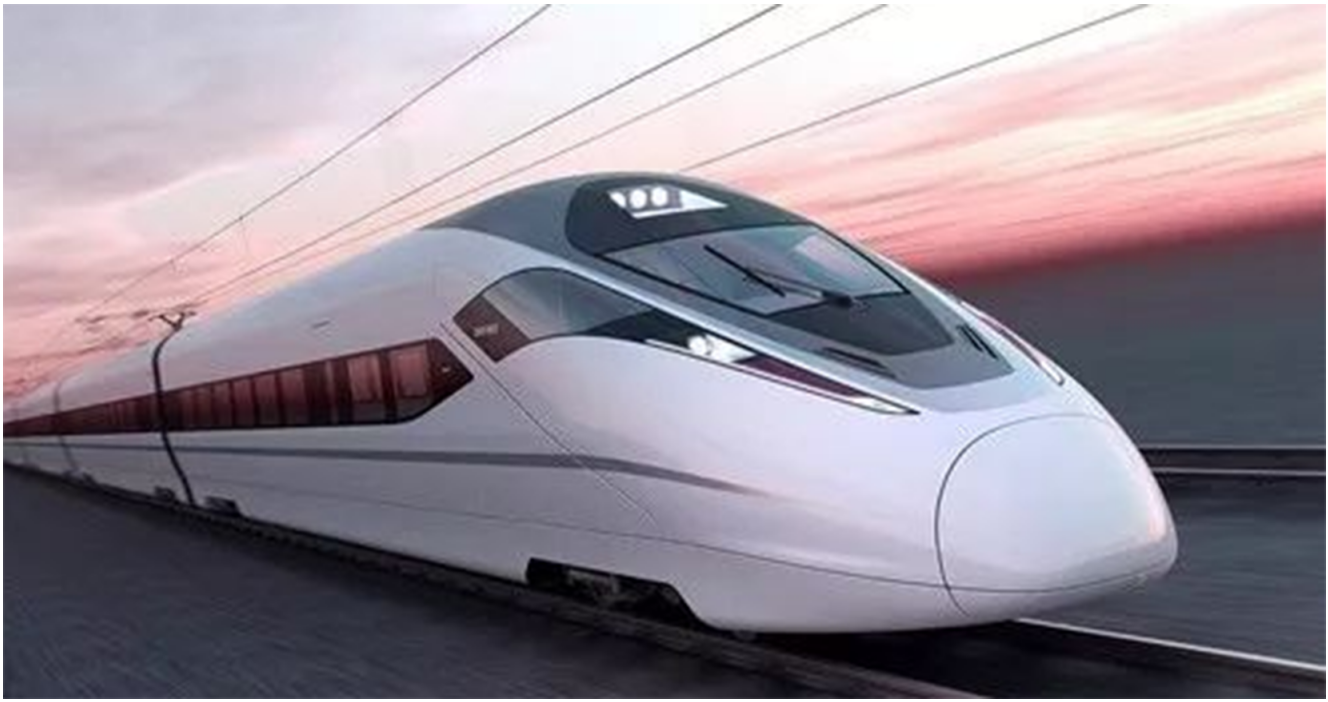
\includegraphics[width=0.3\linewidth]{picture/screenshot055}
\end{figure}


\fourchoices
{做匀加速直线运动}
{加速度逐渐减小}
{牵引力的功率 $ P=Fv_{m} $}
{牵引力做功 $W=\frac{1}{2} m v_{\mathrm{m}}^{2}-\frac{1}{2} m v_{0}^{2}$}






\gaokaosy

\item
\begin{enumerate}
\item
某实验小组利用图 \subref{2020天津09a} 所示装置测定平抛运动的初速度。把白纸和复写纸叠放一起固定在竖直木板
上,在桌面上固定一个斜面,斜面的底边 $ ab $ 与桌子边缘及木板均平行。每次改变木板和桌边之间
的距离,让钢球从斜面顶端同一位置滚下,通过碰撞复写纸,在白纸上记录钢球的落点。
\begin{figure}[h!]
\centering
\begin{subfigure}{0.4\linewidth}
\centering
\includesvg[width=0.7\linewidth]{picture/svg/GZ-3-tiyou-0772} 
\caption{}\label{2020天津09a}
\end{subfigure}
\begin{subfigure}{0.4\linewidth}
\centering
\includesvg[width=0.135\linewidth]{picture/svg/GZ-3-tiyou-0773} 
\caption{}\label{2020天津09b}
\end{subfigure}
\end{figure}

\begin{enumerate}
\item
为了正确完成实验,以下做法必要的是 \underlinegap 。
\fourchoices
{实验时应保持桌面水平}
{每次应使钢球从静止开始释放}
{使斜面的底边 $ ab $ 与桌边重合}
{选择对钢球摩擦力尽可能小的斜面}

\item 
实验小组每次将木板向远离桌子的方向移动 $ 0.2 \ m $,在白纸上记录了钢球的 $ 4 $ 个落点,相邻两点之间的距离依次为 $ 15.0 \ cm $、$ 25.0 \ cm $、$ 35.0 \ cm $,示意如图 $ b $。重力加速度 $ g=10 \ m/s^{2} $,钢球平抛的初速度为 \underlinegap $ m/s $。

\item 
图 \subref{2020天津09a} 装置中,木板上悬挂一条铅垂线,其作用是 \hfullline 。

\end{enumerate}


\tk{
\begin{enumerate}
\item
AB 
\item 
$ 2 $ 
\item 
方便将木板调整到竖直平面	
\end{enumerate} 
} 





\item 
某实验小组选用以下器材测定电池组的电动势和内阻,要求测量结果尽量准确。


电压表 \qquad (量程 $ 0 \sim 3 \ V $,内阻约为 $ 3 \ k \Omega $ )

电流表 \qquad (量程 $ 0 \sim 0.6 \ A $,内阻约为 $ 1 \ \Omega $ )

滑动变阻器 \qquad ( $ 0 \sim 20 \ \Omega $,额定电流 $ 1 \ A $ )

待测电池组 \qquad (电动势约为 $ 3 \ V $,内阻约为 $ 1 \ \Omega $ )

开关、导线若干

\begin{enumerate}
\item
该小组连接的实物电路如图所示,经仔细检查,发现电路中有一条导线连接不当,这条导线对
应的编号是 \underlinegap 。
\begin{figure}[h!]
\centering
\includesvg[width=0.45\linewidth]{picture/svg/GZ-3-tiyou-0774}
\end{figure}


\item 
改正这条导线的连接后开始实验,闭合开关前,滑动变阻器的滑片 $ P $ 应置于滑动变阻器的
端 \underlinegap (填“$ a $”或者“$ b $”)

\item 
实验中发现调节滑动变阻器时,电流表读数变化明显但电压表读数变化不明显。为了解决这个问题,在电池组负极和开关之间串联一个阻值为 $ 5 \ \Omega $ 的电阻,之后该小组得到了几组电压表读数 $ U $
和对应的电流表读数 $ I $ ,
并作出 $ U-I $ 图像,如图所示。根据图像可知,
电池组的电动势为 \underlinegap $ V $,
内阻为 \underlinegap $ \Omega $。(结果均保留两位有效数字)
\begin{figure}[h!]
\centering
\includesvg[width=0.45\linewidth]{picture/svg/GZ-3-tiyou-0775}
\end{figure}

\end{enumerate}

\tk{
\begin{enumerate}
\item
$ 5 $
\item 
$ a $ 
\item 
$ 2.9 \quad 0.80 $
\end{enumerate} 
} 




\end{enumerate}





\gaokaojs

\item
如图所示,垂直于纸面向里的匀强磁场,磁感应强度 $ B $ 随时间 $ t $ 均匀变化。正方形硬质金属
框 $ abcd $ 放置在磁场中,金属框平面与磁场方向垂直,电阻 $ R=0.1 \ \Omega $,边长 $ l=0.2 \ m $。求:
\begin{enumerate}
\item
在 $ t=0 $ 到 $ t=0.1 \ s $ 时间内,金属框中的感应电动势 $ E $;
\item 
$ t=0.05 \ s $ 时,金属框 $ ab $ 边受到的安培力 $ F $ 的大小和方向;
\item 
在 $ t=0 $ 到 $ t=0.1 \ s $ 时间内,金属框中电流的电功率 $ P $。

\end{enumerate}
\begin{figure}[h!]
\flushright
\begin{subfigure}{0.4\linewidth}
\centering
\includesvg[width=0.4\linewidth]{picture/svg/GZ-3-tiyou-0776} 
\caption{}\label{}
\end{subfigure}
\begin{subfigure}{0.4\linewidth}
\centering
\includesvg[width=0.6\linewidth]{picture/svg/GZ-3-tiyou-0777} 
\caption{}\label{}
\end{subfigure}
\end{figure}

\banswer{
\begin{enumerate}
\item
$E=0.08 \ V$
\item 
$F=0.016 \ N$方向垂直于 $a b$ 向左。
\item 
$P=0.064 \ W$
\end{enumerate}
}





\item
长为 $ l $ 的轻绳上端固定,下端系着质量为 $ m_{1} $ 的小球 $ A $,处于静止状态。$ A $ 受到一个水平瞬时
冲量后在竖直平面内做圆周运动,恰好能通过圆周轨迹的最高点。当 $ A $ 回到最低点时,质量为 $ m_{2} $ 的小
球 $ B $ 与之迎面正碰,碰后 $ A $、$ B $ 粘在一起,仍做圆周运动,并能通过圆周轨迹的最高点。不计空气阻力,重力加速度为 $ g $,求:
\begin{enumerate}
\item
$ A $ 受到的水平瞬时冲量 $ I $ 的大小;
\item 
碰撞前瞬间 $ B $ 的动能 $ E_{k} $ 至少多大?
\end{enumerate}


\banswer{
\begin{enumerate}
\item
$I=m_{1} \sqrt{5 g l}$
\item 
$E_{\mathrm{k}}=\frac{5 g l\left(2 m_{1}+m_{2}\right)^{2}}{2 m_{2}}$
\end{enumerate}
}





\newpage
\item
多反射飞行时间质谱仪是一种测量离子质量的新型实验仪器,其基本原理如图所示,从离子
源 $ A $ 处飘出的离子初速度不计,经电压为 $ U $ 的匀强电场加速后射入质量分析器。质量分析器由两个反
射区和长为 $ l $ 的漂移管(无场区域)构成,开始时反射区 $ 1 $、$ 2 $ 均未加电场,当离子第一次进入漂移管
时,两反射区开始加上电场强度大小相等、方向相反的匀强电场,其电场强度足够大,使得进入反射
区的离子能够反射回漂移管。离子在质量分析器中经多次往复即将进入反射区 $ 2 $ 时,撤去反射区的电
场,离子打在荧光屏 $ B $ 上被探测到,可测得离子从 $ A $ 到 $ B $ 的总飞行时间。设实验所用离子的电荷量均
为 $ q $,不计离子重力。
\begin{enumerate}
\item
求质量为 $ m $ 的离子第一次通过漂移管所用的时间 $ T_{1} $;
\item 
反射区加上电场,电场强度大小为 $ E $,求离子能进入反射区的最大距离 $ x $;
\item 
已知质量为 $ m_{0} $ 的离子总飞行时间为 $ t_{0} $,待测离子的总飞行时间为 $ t_{1} $,两种离子在质量分析器中
反射相同次数,求待测离子质量 $ m_{1} $。



\end{enumerate}
\begin{figure}[h!]
\flushright
\includesvg[width=0.85\linewidth]{picture/svg/GZ-3-tiyou-0778}
\end{figure}

\tk{
\begin{enumerate}
\item
$T_{1}=l\sqrt{\frac{m}{2 q U}}$
\item 
$x=\frac{U}{E}$
\item 
$m_{1}=\left(\frac{t_{1}}{t_{0}}\right)^{2} m_{0}$
\end{enumerate}
} 




\end{enumerate}

